\documentclass[a4paper, 11pt, ngerman, fleqn]{article}
\usepackage[utf8]{inputenc}
\usepackage{babel}
\usepackage{ngerman}
\usepackage{coordsys,logsys,color}
\usepackage{german,fancyhdr}
\usepackage{hyperref}
\usepackage{texdraw}
\input{txdtools}

\NeedsTeXFormat{LaTeX2e}
\ProvidesPackage{hyperref}
\definecolor{darkblue}{rgb}{0,0,.6}
\hypersetup{pdftex=false, colorlinks=true, breaklinks=true, linkcolor=darkblue, menucolor=darkblue, pagecolor=darkblue, urlcolor=darkblue, citecolor=darkblue}

\pagestyle{fancy}

\renewcommand{\familydefault}{cmss}

\definecolor{fgcgray}{rgb}{0.4, 0.4, 0.4}
\definecolor{warning}{rgb}{0.9, 0.1, 0.0}
\definecolor{bgctitle}{rgb}{0.5, 0.5, 0.5}
\definecolor{fgctitle}{rgb}{0.95, 0.95, 0.95}
\newcommand{\titlefont}[1]{\textcolor{fgctitle}{\fontfamily{cmss}\fontseries{bx}\fontshape{n}\fontsize{20.48}{0pt} \selectfont #1}}
\newcommand{\inversetitlefont}[1]{\textcolor{bgctitle}{\fontfamily{cmss}\fontseries{bx}\fontshape{n}\fontsize{20.48}{0pt} \selectfont #1}}

\addtolength{\oddsidemargin}{-1.0cm}
\addtolength{\evensidemargin}{-1.0cm}
\addtolength{\headwidth}{2.0cm}
\addtolength{\textwidth}{2.0cm}

\setlength{\parindent}{0cm}

\renewcommand{\labelitemi}{$\circ$}
\renewcommand{\labelitemii}{$\diamond$}

\newcommand{\spaceline}[1][8pt]{\vskip #1}
\newcommand{\comment}[1]{\spaceline[5pt] \textcolor{fgcgray}{\scriptsize #1} \spaceline[15pt]}
\newcommand{\attrname}[1]{\textcolor{fgcgray}{\scriptsize #1}}


\makeatletter

\newcommand*{\project}[1]{\gdef\@project{#1}}
\newcommand*{\version}[1]{\gdef\@version{#1}}
\newcommand*{\home}[1]{\gdef\@home{#1}}
\newcommand*{\homeref}[1]{\gdef\@homeref{#1}}
\newcommand*{\prerequisite}[1]{\gdef\@prerequisite{#1}}
\newcommand*{\prerequisiteref}[1]{\gdef\@prerequisiteref{#1}}

\def\@maketitle{
  %\begin{titlepage}
  \begin{center}
    \colorbox{bgctitle}{
      \parbox{\textwidth}{
        \spaceline
        \centering{\titlefont{\@title}}
        \par
        \spaceline
      }
    }
    \colorbox{white}{
      \parbox{\textwidth}{
        \spaceline
        \centering{\inversetitlefont{\@project}}
        \par
        \spaceline
      }
    }
  \end{center}
  \spaceline[1.5em] {
    \begin{flushright}
    \begin{tabular}[t]{rl}
      \attrname{Projekt:} & \@project ~ \@version \\
      \attrname{Autoren:} & \@author \\
      \attrname{letzte "Anderung:} & \@date
    \end{tabular}
    \end{flushright}
    \par
  }
  \spaceline[5.5em]
  %\end{titlepage}
}

\setcounter{secnumdepth}{4}
\setcounter{tocdepth}{4}
	 
\newcounter{subsubsubsection}[subsubsection]
\def\subsubsubsectionmark#1{}
\def\thesubsubsubsection{\thesubsubsection .\arabic{subsubsubsection}}
\def\subsubsubsection{\@startsection{subsubsubsection}{4}{\z@}{-3.25ex plus -1 ex minus -.2ex}{1.5ex plus .2ex}{\normalsize\bf}}
\def\l@subsubsubsection{\@dottedtocline{4}{4.8em}{4.2em}}

\makeatother

\everytexdraw{
  \drawdim cm \linewd 0.01
  \arrowheadtype t:T
  \arrowheadsize l:0.2 w:0.2
  \setgray 0.5
}

\newcommand{\xheight}{0.6}
\newcommand{\xlength}{0.6}
\newcommand{\yheighta}{1.0}
\newcommand{\yheightb}{0.8}
\newcommand{\yheightc}{0.6}
\newcommand{\yheightd}{0.5}
\newcommand{\yheighte}{0.4}
\newcommand{\yheightf}{0.35}

\newcommand{\xhline}{\rlvec({\xlength} 0)}
\newcommand{\xharrow}{\ravec(0.7 0)}
\newcommand{\xnext}{%\rlvec(0.05 0) \lpatt(0.04 0.04) \rlvec(0.15 0) \lpatt()
}

\newcommand{\xtext}[3][\xheight]{
  \bsegment
    \bsegment
      \setsegscale 0.5
      \textref h:L v:C  \htext({\xheight} -0.1){#3}
    \esegment
    \setsegscale 0.5 \lvec(0 #1)
    \setsegscale 1
    \rlvec(#2 0) \rlvec(0 -#1) \rlvec(-#2 0) \lvec(0 0)
    \savepos(#2 0)(*@x *@y)
  \esegment
  \move(*@x *@y)
}

\newcommand{\bxtext}[3][\xheight]{
  \setgray{0.1}
  \linewd{0.026}
  \xtext[\xheight]{#2}{#3}
  \linewd{0.01}
  \setgray{0.5}
}

\newcommand{\xstartpage}{\bxtext{2.1}{Startseite}}
\newcommand{\xmainpage}{\bxtext{2.3}{Hauptseite}}
\newcommand{\xusermenu}{\bxtext{2.9}{Benutzermenu}}
\newcommand{\xgamelist}{\bxtext{2.2}{Spieleliste}}
\newcommand{\xportfolio}{\bxtext{2.0}{Portfolio}}
\newcommand{\xaccount}{\xtext{3.8}{Kennung per \textsl{eMail}}}


\begin{document}
  %!TEX root = Pflichtenheft.tex

\title{Pflichtenheft Praktikum Softwareentwurf WS 2011/12}
\project{Rechnungssystem}
\author{Sascha Ebert () - Teamleiter\\&Morris Jobke ()\\&Markus Ast ()\\&Robert Schönherr ()\\&Michael Hertel ()}
\tutor{Dr. Frank Seifert}
\groupnumber{1}

\maketitle \newpage
  \tableofcontents \newpage
  %!TEX root = Pflichtenheft.tex

\section{Zielbestimmungen}



\subsection{Musskriterien}

\begin{itemize}
	\item Rechnungssystem für Selbständige, welches Endjahresbilanzen bzw. Gewinn-Verlust-Überschussrechnungen bereitstellt
	\item Rechnungen können im PDF-Format ausgegeben werden
	\item Anpassbare Rechnungs-PDFs durch vom Nutzer vorgegebene Latex oder HTML-Templates
	\item Erstellen und Verwalten von Rechnungs-Repositorys zum Verwalten der Rechnungen
	\item Bereitstellung eines GDK-Frontends
\end{itemize}

\subsection{Sollkriterien}

\begin{itemize}
	\item Ausgegebene Rechnungs-PDFs werden digital signiert
\end{itemize}

\subsection{Abgrenzungskriterien}

\begin{itemize}
	\item Rechnungssystem beachtet keine Steuern
	\item Rechnungssystem nicht für Unternehmen geeignet
\end{itemize} \newpage
  %!TEX root = Pflichtenheft.tex

\section{Produkteinsatz}


\subsection{Anwendungsbereiche}

Das Rechnungssystem soll Kleinunternehmern eine einfache und effiziente Verwaltung und Erstellung von Rechnungen ermöglichen. 

\subsection{Zielgruppen}

Das Projekt richtet sich an Kleinunternehmer, welche Rechnungen erstellen und verwalten müssen. 

Grundlegende Computerkenntnisse und auch grundlegende Kentnisse von HTML bzw. Latex sind, für die Erstellung eigener Templates, von Vorteil, aber nicht zwingend notwendig.

Des Weiteren soll eine Grundlage für weiterreichende Projekte geschaffen werden, welche von anderen Entwicklern genutzt werden kann.

\subsection{Systemvoraussetzungen, Hardware}
Es werden folgende Komponenten benötigt:
\begin{itemize}
	\item PC mit Linux-, oder Mac-Betriebssystem
	\item Editor oder ähnliche Anwendung zum Bearbeiten der Templates (optional? -> Standard-Templates?)
	\item TeX-Distribution (optional)
	\item Sqlite (optional)
\end{itemize}

\subsection{Betriebsbedingungen}
Die Anwendung soll sich nicht stark von den Betriebsbedingungen anderer typischer Verwaltungssoftware unterscheiden:

\begin{itemize}
	\item Betriebszeit: bei Bedarf
	\item wartungsfrei
	\item die Sicherung der Daten obliegt dem Nutzer
\end{itemize}
 \newpage
  %!TEX root = Pflichtenheft.tex

\section{Produktübersicht}

% \begin{itemize}
% 	\item UML-Diagramme zu den Use-Cases hinzufügen
% \end{itemize}

% Repo erstellen und konfigurieren (Template, Rechnungsnummern, ...)
% Rechnung ausfüllen und erstellen (PDF, HTML, ...)
% Verwaltung der Rechnungen (offene Rechnungen, Statistiken, Analsye...)

% [Benutzer]-(Rechnung anlegen)
% [Benutzer]-(Rechnungsstatus ausgeben)
% [Benutzer]-(Rechnungsattribute bearbeiten)
% [Benutzer]-(Rechnung rendern)
% [Benutzer]-(Template konfigurieren)
% [Benutzer]-(Rechnungen durchsuchen)
% [Benutzer]-(Rechnung löschen)
% (Rechnung anlegen)<(Rechnungsattribute eingeben)
% (Rechnungsattribute bearbeiten)<(Rechnungsattribute eingeben)
% (Template konfigurieren)<(Platzhalter eintragen)
% http://yuml.me/5ed27f7e

\begin{center}
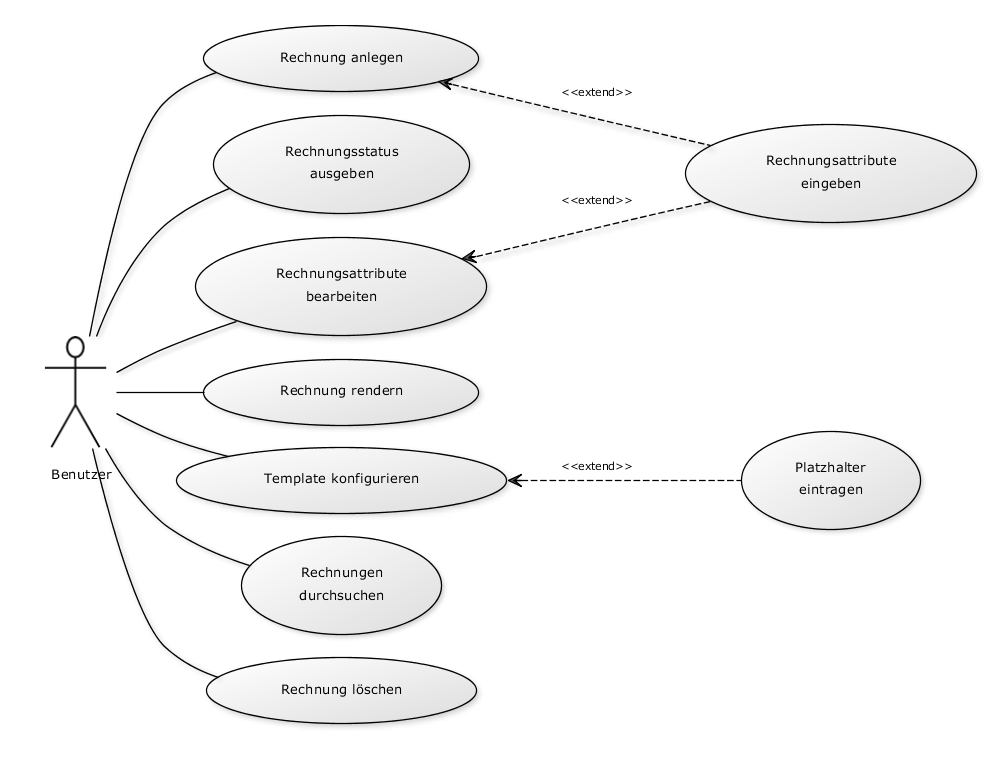
\includegraphics[width=0.8\textwidth]{03-Use-Case.png}
\end{center} \newpage
  %!TEX root = Pflichtenheft.tex

\section{Produktleistungen}

\begin{description}
	\item[/L100/]
		\textit{Genauigkeit:}
			Jegliche Geldbeträge im Programm sind auf 2 Nachkommastellen genau.
\end{description}

\begin{description}
	\item[/L200/]
		\textit{Unterstützung für korrekte Templates:}
			Verwendet der Programmnutzer ein unvollständiges Template mit fehlenden Platzhaltern erhält er eine Warnung.
\end{description}

\begin{description}
	\item[/L300/]
		\textit{Akkumulation:}
			Bei fehlerhaften Eingaben erhält der Benutzer eine aussagekräftige Fehlermeldung.
\end{description}

	%\item Validierung
 \newpage
  \section{Qualit\"atsanforderungen}



\begin{center}
 \begin{tabular}{l|c|c|c|c}
  ~ & sehr wichtig & wichtig & weniger wichtig & unwichtig\\
  \hline \hline
  \textit{Robustheit}~ &  ~ ~ ~ & \textbf{X}~ &  ~ ~ ~ &  ~ ~ ~ \\
  \hline
  \textit{Zuverl\"assigkeit}~ & \textbf{X}~ &  ~ ~ ~ &  ~ ~ ~ &  ~ ~ ~ \\
  \hline
  \textit{Korrektheit}~ & \textbf{X}~ &  ~ ~ ~ &  ~ ~ ~ &  ~ ~ ~ \\
  \hline
  \textit{Benutzungsfreundlichkeit}~ &  ~ ~ ~ & \textbf{X}~ &  ~ ~ ~ &  ~ ~ ~ \\
  \hline
  \textit{Effizienz}~ &  ~ ~ ~  &  ~ ~ ~ & \textbf{X}~ &  ~ ~ ~ \\
  \hline
  \textit{Portierbarkeit}~ &  ~ ~ ~ &  ~ ~ ~ & \textbf{X}~ &  ~ ~ ~ \\
  \hline
  \textit{Kompatibilit\"at}~ &  ~ ~ ~ & \textbf{X}~ &  ~ ~ ~ &  ~ ~ ~ \\
 \end{tabular}
\end{center}
 \newpage
  %!TEX root = Pflichtenheft.tex

\section{Testszenarien und Testf\"alle}



\begin{description}
  \item[/T0010/]
    \textit{Erstellen einer Rechnung mit einem HTML-Template:}
   Es wird zun\"achst ein g\"ultiges HTML-Template erstellt. Dieses wird dann mit zuvor in das Rechnungssystem eigegebenen Testdaten gef\"ullt. Das dadurch entstandene Rechnungs-PDF wird zuletzt auf Vollst\"andigkeit und Korrektheit \"uberpr\"uft.
	\begin{itemize}
   		\item Erstellen einer Rechnung mit einem HTML-Template -> vollständige Rechnung als PDF
		\item Erstellen einer Rechnung mit einem Latex-Template -> vollständige Rechnung als PDF
		\item Testen des Programms auf Reaktion auf ein defektes/unvollständiges Template -> Fehlermeldung
		\item Berechnen der Endjahresbilanz / Gewinn-Verlust-Überschussrechnung ->korrekte Ausgabe
		\item Anlegen mehrerer Rechnungs-Repositorys -> mehrere Repositorys mit jeweils einer DB
   \end{itemize}
\end{description}


 \newpage
  \section{Entwicklungsumgebung}


\subsection{Software}

\begin{itemize}
  \item Plattform
    \begin{itemize}

    \end{itemize}
  \item Tools
    \begin{itemize}
  
    \end{itemize}

\end{itemize}

\subsection{Hardware}

\begin{itemize}

\end{itemize}

\subsection{Orgware}

\begin{itemize}
  
\end{itemize}
 \newpage
  %!TEX root = Pflichtenheft.tex

\section{Erg\"anzungen}

 \newpage
  %!TEX root = Pflichtenheft.tex

\section{Glossar}


\begin{itemize}
	\item Template = eine Mustervorlage bei der in dafür vorgesehene Bereiche Daten eingefügt werden können
	\item Repository = ein verwaltetes Verzeichnis in welchem digitale Daten gespeichert werden können
	\item ...?
\end{itemize}


\end{document}
